\documentclass[10pt]{article}
\usepackage[T1]{fontenc}
\usepackage{lmodern}
\usepackage[margin=0.78in]{geometry}
\usepackage{microtype}
\usepackage{amsmath,amssymb}
\usepackage{graphicx}
\usepackage{booktabs,array,multirow}
\usepackage[table]{xcolor}
\usepackage{siunitx}
\usepackage{pdflscape}
\usepackage{hyperref}
\usepackage{fancyhdr}
\usepackage{enumitem}
\usepackage{caption}
\usepackage{parskip}

\definecolor{navy}{HTML}{153B5B}
\definecolor{blue}{HTML}{1768AC}
\definecolor{red}{HTML}{D1495B}
\definecolor{teal}{HTML}{2A9D8F}
\definecolor{softgray}{HTML}{F3F5F7}
\hypersetup{colorlinks=true,linkcolor=navy,urlcolor=blue,pdftitle={PySR on Fully Observable NeuronBench}}
\captionsetup{font=small,labelfont=bf}
\setlist[itemize]{leftmargin=1.4em,itemsep=0.25em,topsep=0.25em}
\pagestyle{fancy}
\fancyhf{}
\fancyhead[L]{\small\color{navy} PySR on Fully Observable NeuronBench}
\fancyhead[R]{\small\color{gray} 1M evaluations, 3 seeds}
\fancyfoot[C]{\thepage}
\renewcommand{\headrulewidth}{0.3pt}
\newcommand{\methodA}{\textcolor{blue}{Vanilla PySR}}
\newcommand{\methodB}{\textcolor{red}{Evolved 538190}}

\begin{document}

\begin{center}
{\color{navy}\LARGE\bfseries PySR on Fully Observable NeuronBench}\\[0.55em]
{\large A controlled symbolic-regression comparison of vanilla PySR and evolved run 538190}\\[0.8em]
{\small Six deterministic worlds $\times$ two methods $\times$ three seeds; $10^6$ maximum evaluations per fit}\\[0.25em]
{\small Report generated 18 August 2026}
\end{center}

\vspace{0.6em}
\noindent\colorbox{softgray}{\parbox{0.96\linewidth}{
\textbf{Bottom line.} Vanilla PySR produced the only numerically recovered vector field
(Na-fatigue, seed 1; held-out NRMSE $3.44\!\times\!10^{-7}$), but neither
method achieved literal symbolic identity. Across all 18 paired fits the result was a
\textbf{9--9 tie}. Evolved 538190 was modestly better on affine-calibrated shape error,
as expected from its affine-invariant loss, but it did not improve full physical-dynamics recovery.
}}

\section{Question and reduction}

NeuronBench\footnote{\url{https://github.com/murphyk/neuronbench}, pinned at
\texttt{c354622458c460b419cab821d482c879f0578377}. The benchmark is introduced in
\url{https://arxiv.org/abs/2608.09696}.} normally combines active experiment design,
partially observed gating state, and mechanistic model discovery. This study deliberately removes
the first two difficulties. For every deterministic world, the regressor observes injected current
$I_{\rm ext}$, membrane voltage $V$, and every composite channel-open fraction $\phi_c$ from the
benchmark's Eq.~(32). The target is the exact voltage vector field
\begin{equation}
\dot V = I_{\rm ext} - \sum_c g_c\,\phi_c\,(V-E_c).
\label{eq:vectorfield}
\end{equation}
The result is six ordinary noiseless scalar SR problems. The composite features remain mechanistic:
for example, $\phi_{\rm Na}=m_{\rm Na}^3h_{\rm Na}$ and
$\phi_{\rm K}=n_{\rm K}^4$; in Na-fatigue,
$\phi_{\rm Na}=m_{\rm Na}^3h_{\rm Na}s_{\rm Na}$ includes the slow inactivation state.

\begin{table}[h]
\centering
\caption{World-specific term added to the common Na/K/leak current balance.}
\small
\begin{tabular}{lll}
\toprule
World & Additional observable / state change & Additional term in $\dot V$ \\
\midrule
Z-rebound & $\phi_Z=m_Z^2h_Z$ & $-4\phi_Z(V-120)$ \\
H-sag & $\phi_h=m_h$ & $-5\phi_h(V+30)$ \\
Na-fatigue & $\phi_{\rm Na}$ includes $s_{\rm Na}$ & none beyond modified $\phi_{\rm Na}$ \\
Ca-rebound & $\phi_T=m_T^2h_T$ & $-3.2\phi_T(V-120)$ \\
D-type & $\phi_D=m_Dh_D$ & $-9\phi_D(V+77)$ \\
Textbook-M & $\phi_M=m_M$ & $-2.5\phi_M(V+77)$ \\
\bottomrule
\end{tabular}
\end{table}

\section{Experimental protocol}

\begin{itemize}
\item \textbf{Data.} 1,024 training and 16,384 held-out scrambled-Sobol states per world,
covering $I_{\rm ext}\in[-40,20]$, $V\in[-95,60]$, and each $\phi_c\in[0,1]$.
Targets are analytic evaluations of Eq.~\eqref{eq:vectorfield}---there is no noise or numerical differentiation.
\item \textbf{Shared search settings.} Binary operators $\{+,-,\times\}$, no unary operators,
15 populations of 33 members, maximum size 35, Float64 arithmetic, deterministic serial execution,
and $10^6$ maximum evaluations. Target RMS scaling is inverted before every reported error.
\item \textbf{Only treatment difference.} Evolved 538190 replaces PySR's mutation, selection,
survival, and loss with the saved bundle from \texttt{runs/538190}. All data, seeds, and search
hyperparameters are otherwise identical.
\item \textbf{Assessment.} For each run, the reported error is the lowest held-out NRMSE attained
anywhere on the discovered Pareto frontier (an oracle assessment of the frontier, not test-set model selection).
Numerical recovery means NRMSE $\leq10^{-6}$; near-exact means $\leq10^{-3}$.
Exact symbolic equality is checked separately with SymPy.
\end{itemize}

\section{Aggregate results}

\begin{table}[h]
\centering
\caption{Overall comparison across 18 fits per method. Lower NRMSE is better.}
\begin{tabular}{lrrrr}
\toprule
Method & Recovered & Exact symbolic & Median raw NRMSE & Median affine-calibrated NRMSE \\
\midrule
\methodA & 1/18 & 0/18 & $4.09\!\times\!10^{-3}$ & $4.02\!\times\!10^{-3}$ \\
\methodB & 0/18 & 0/18 & $4.63\!\times\!10^{-3}$ & $3.51\!\times\!10^{-3}$ \\
\bottomrule
\end{tabular}
\end{table}

The raw comparison does not support an overall improvement from 538190. Vanilla has the lower
median raw error ($4.09\!\times\!10^{-3}$ versus $4.63\!\times\!10^{-3}$)
and the only strict recovery. The paired win count is exactly
9 evolved to 9 vanilla. The secondary calibrated-shape
metric favors 538190 ($3.51\!\times\!10^{-3}$ versus
$4.02\!\times\!10^{-3}$), which is consistent with its custom loss:
that loss scores an affine correction $a f(x)+b$ internally, while the physical equation must itself
recover scale and offset.

\begin{table}[h]
\centering
\caption{Best and median raw frontier error over three seeds. ``Winner'' compares medians.}
\small
\begin{tabular}{lrrrrrl}
\toprule
& GT & \multicolumn{2}{c}{Vanilla PySR} & \multicolumn{2}{c}{Evolved 538190} & \\
\cmidrule(lr){3-4}\cmidrule(lr){5-6}
World & complexity & best & median & best & median & winner \\
\midrule
Z-rebound & 31 & $3.38\!\times\!10^{-3}$ & $3.46\!\times\!10^{-3}$ & $3.12\!\times\!10^{-3}$ & $3.66\!\times\!10^{-3}$ & Vanilla \\
H-sag & 31 & $3.47\!\times\!10^{-3}$ & $3.55\!\times\!10^{-3}$ & $1.68\!\times\!10^{-3}$ & $3.74\!\times\!10^{-3}$ & Vanilla \\
Na-fatigue & 23 & $3.44\!\times\!10^{-7}$ & $3.05\!\times\!10^{-5}$ & $1.00\!\times\!10^{-4}$ & $1.73\!\times\!10^{-3}$ & Vanilla \\
Ca-rebound & 31 & $4.28\!\times\!10^{-3}$ & $9.79\!\times\!10^{-3}$ & $3.92\!\times\!10^{-3}$ & $8.58\!\times\!10^{-3}$ & Evolved \\
D-type & 31 & $4.00\!\times\!10^{-3}$ & $4.17\!\times\!10^{-3}$ & $7.86\!\times\!10^{-4}$ & $5.34\!\times\!10^{-3}$ & Vanilla \\
Textbook-M & 31 & $3.85\!\times\!10^{-3}$ & $5.35\!\times\!10^{-3}$ & $6.55\!\times\!10^{-3}$ & $6.76\!\times\!10^{-3}$ & Vanilla \\
\bottomrule
\end{tabular}
\end{table}

\begin{figure}[p]
\centering
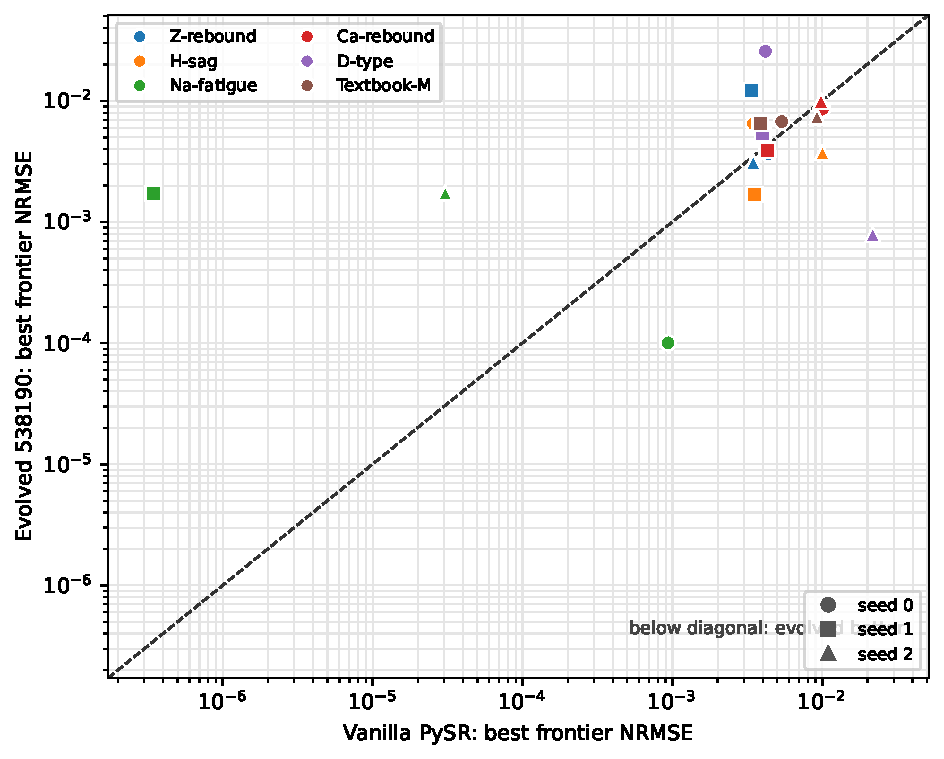
\includegraphics[width=0.83\linewidth]{neuronbench_pysr_fully_observable_assets/paired_raw.pdf}
\caption{Per-seed comparison of the best equation anywhere on each discovered frontier.
Markers encode seed and colors encode world. The 9--9 split around the diagonal shows that
neither method is consistently better.}
\end{figure}

\begin{landscape}
\begin{figure}[p]
\centering
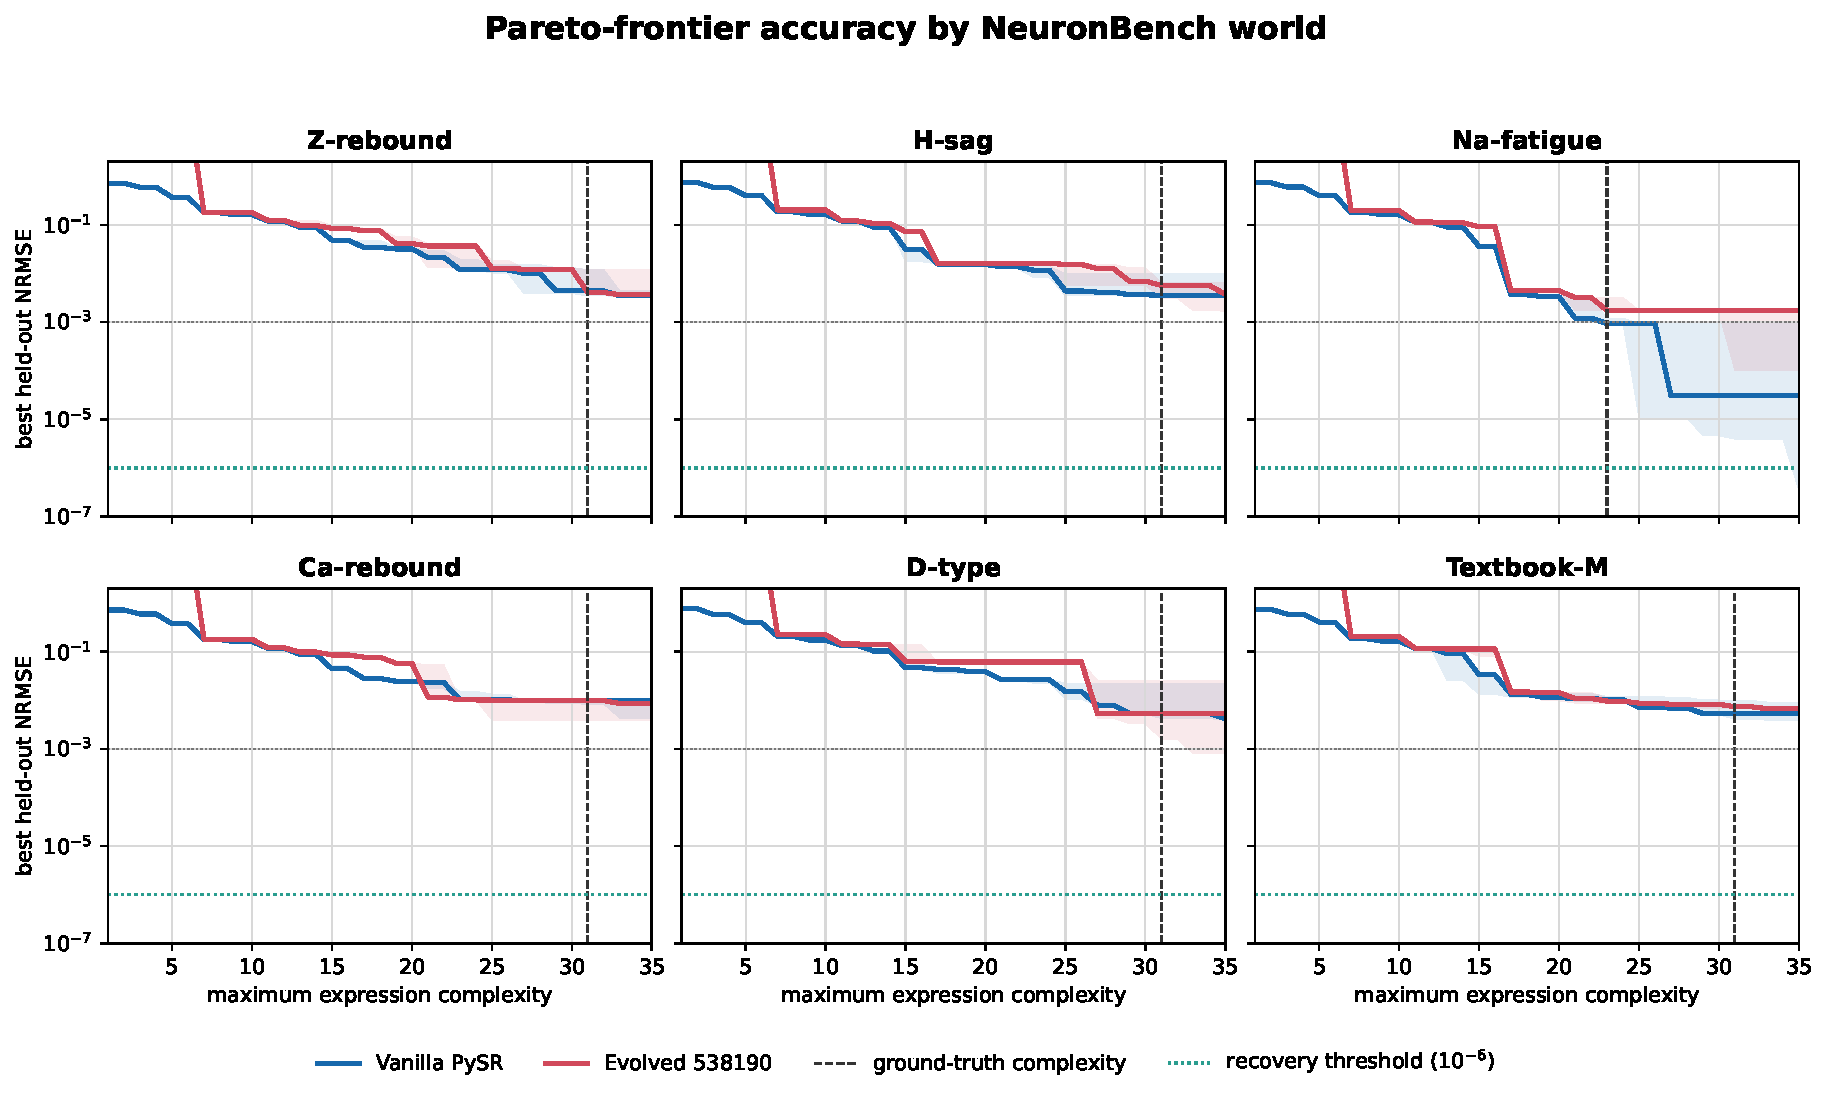
\includegraphics[width=0.97\linewidth]{neuronbench_pysr_fully_observable_assets/frontier_grid.pdf}
\caption{Held-out accuracy along the discovered Pareto frontiers. Solid curves are the median
best-so-far envelope over three seeds; shaded bands span the seedwise minimum to maximum.
The vertical dashed line is the reference ground-truth complexity. The horizontal teal line
is the strict numerical-recovery threshold. Na-fatigue is the only world to cross it.}
\end{figure}
\end{landscape}

\section{What the one recovered run found}

Vanilla PySR's Na-fatigue seed-1 frontier contains a complexity-35 expression with held-out
NRMSE $3.436\!\times\!10^{-7}$. It is not literally identical under symbolic
simplification, but expanding its redundant tree exposes an extremely accurate coefficient match:
\begin{align}
\dot V_{\rm true} ={}& I_{\rm ext} -36\phi_KV-2772\phi_K-120\phi_{\rm Na}V
 +6000\phi_{\rm Na}-0.3V-16.32,\\
\widehat{\dot V} ={}& 1.000045I_{\rm ext}-35.999901\phi_KV-2771.9985\phi_K
 -119.99995\phi_{\rm Na}V \notag\\
&+6000.0037\phi_{\rm Na}-0.300082V-16.322334.
\end{align}
Thus the numerical recovery is scientifically meaningful, although the search used 12 more nodes
than the compact reference expression (35 versus 23) and did not reproduce exact floating constants.

\begin{table}[h]
\centering
\caption{Expanded coefficients for the recovered Na-fatigue run.}
\small
\begin{tabular}{lrrr}
\toprule
Term & truth & discovered & relative error \\
\midrule
$I_{\rm ext}$ & $1$ & $1.000045$ & $4.5\times10^{-5}$ \\
$\phi_KV$ & $-36$ & $-35.999901$ & $2.8\times10^{-6}$ \\
$\phi_K$ & $-2772$ & $-2771.9985$ & $5.4\times10^{-7}$ \\
$\phi_{\rm Na}V$ & $-120$ & $-119.99995$ & $4.2\times10^{-7}$ \\
$\phi_{\rm Na}$ & $6000$ & $6000.0037$ & $6.2\times10^{-7}$ \\
$V$ & $-0.3$ & $-0.300082$ & $2.7\times10^{-4}$ \\
constant & $-16.32$ & $-16.322334$ & $1.4\times10^{-4}$ \\
\bottomrule
\end{tabular}
\end{table}

\section{Best evolved near-miss}

The strongest evolved result is D-type seed 2 (NRMSE $7.862\!\times\!10^{-4}$).
After expansion,
\begin{align}
\widehat{\dot V}_{538190} ={}&0.997137 I_{\rm ext}-9.18239\phi_DV-695.786\phi_D
-36.1745\phi_KV-2775.07\phi_K \notag\\
&-120.193\phi_{\rm Na}V+5997.49\phi_{\rm Na}-11.5219.
\end{align}
It identifies all three gated-current structures and gets their coefficients close, but it omits the
leak slope $-0.3V$ and shifts the constant (truth $-16.32$). This is exactly the distinction between
shape recovery and a correct physical vector field that the raw-versus-calibrated evaluation is meant
to expose.

\section{Conclusions and limitations}

\begin{enumerate}[leftmargin=1.6em,itemsep=0.35em]
\item \textbf{Vanilla PySR can solve at least one simplified NeuronBench world.} It numerically
recovers Na-fatigue in one of three seeds, with coefficient errors mostly below $10^{-4}$ relative.
\item \textbf{Run 538190 does not improve strict recovery at this budget.} It has zero strict
recoveries, a slightly worse raw median, and an exactly tied paired win count.
\item \textbf{538190 does improve affine-calibrated shape modestly.} This aligns with its evolved
loss rather than demonstrating better recovery of physically scaled dynamics.
\item \textbf{This is intentionally not the original benchmark task.} Composite open fractions
are supplied, all states are sampled directly, and the study learns only $\dot V$. It does not test
active design, recovery of gate ODEs, latent-state inference, or trajectory forecasting.
\item \textbf{Three seeds are enough for a demo, not a fine-grained ranking.} The broad seed bands
and 9--9 paired split argue against claiming a small algorithmic advantage either way.
\end{enumerate}

\begin{landscape}
\section{Appendix: all 36 best-frontier errors}
\begin{table}[h]
\centering
\caption{Held-out raw NRMSE of the closest equation anywhere on each run's frontier.
Green marks strict recovery; blue marks near-exact ($\leq10^{-3}$).}
\normalsize
\setlength{\tabcolsep}{9pt}
\begin{tabular}{lrrrrrr}
\toprule
& \multicolumn{3}{c}{Vanilla PySR} & \multicolumn{3}{c}{Evolved 538190} \\
\cmidrule(lr){2-4}\cmidrule(lr){5-7}
World & seed 0 & seed 1 & seed 2 & seed 0 & seed 1 & seed 2 \\
\midrule
Z-rebound & $4.38\!\times\!10^{-3}$ & $3.38\!\times\!10^{-3}$ & $3.46\!\times\!10^{-3}$ & $3.66\!\times\!10^{-3}$ & $1.21\!\times\!10^{-2}$ & $3.12\!\times\!10^{-3}$ \\
H-sag & $3.47\!\times\!10^{-3}$ & $3.55\!\times\!10^{-3}$ & $1.00\!\times\!10^{-2}$ & $6.50\!\times\!10^{-3}$ & $1.68\!\times\!10^{-3}$ & $3.74\!\times\!10^{-3}$ \\
Na-fatigue & \cellcolor{blue!10}$9.34\!\times\!10^{-4}$ & \cellcolor{green!16}\textbf{$3.44\!\times\!10^{-7}$} & \cellcolor{blue!10}$3.05\!\times\!10^{-5}$ & \cellcolor{blue!10}$1.00\!\times\!10^{-4}$ & $1.73\!\times\!10^{-3}$ & $1.74\!\times\!10^{-3}$ \\
Ca-rebound & $1.00\!\times\!10^{-2}$ & $4.28\!\times\!10^{-3}$ & $9.79\!\times\!10^{-3}$ & $8.58\!\times\!10^{-3}$ & $3.92\!\times\!10^{-3}$ & $9.99\!\times\!10^{-3}$ \\
D-type & $4.17\!\times\!10^{-3}$ & $4.00\!\times\!10^{-3}$ & $2.17\!\times\!10^{-2}$ & $2.57\!\times\!10^{-2}$ & $5.34\!\times\!10^{-3}$ & \cellcolor{blue!10}$7.86\!\times\!10^{-4}$ \\
Textbook-M & $5.35\!\times\!10^{-3}$ & $3.85\!\times\!10^{-3}$ & $9.23\!\times\!10^{-3}$ & $6.76\!\times\!10^{-3}$ & $6.55\!\times\!10^{-3}$ & $7.38\!\times\!10^{-3}$ \\
\bottomrule
\end{tabular}
\end{table}

\vspace{1em}
\begin{minipage}{0.9\linewidth}
\subsection*{Reproducibility}
{\small NeuronBench was installed into the \texttt{meta\_sr} conda environment at the pinned commit above.
The complete frontiers and metrics are in
\path{reports/neuronbench_pysr_fully_observable.results.json}. The experiment runner is
\path{scripts/neuronbench_fully_observable.py} and this report is regenerated by
\path{scripts/build_neuronbench_latex_report.py}. SLURM array job 142502 completed all 36 tasks
without a nonzero exit or traceback.}
\end{minipage}
\end{landscape}

\end{document}
